\chapter{Newton's law solutions}
\begin{abox}
	Practice set 1 solutions
	\end{abox}
\begin{enumerate}
\begin{minipage}{\textwidth}
	\item The trajectory on the $z p_{z}$ - plane (phase-space trajectory) of a ball bouncing perfectly elastically off a hard surface at $z=0$ is given by approximately by (neglect friction):
	\exyear{NET JUNE 2011}
\end{minipage}
\begin{tasks}(2)
	\task[\textbf{A.}]\begin{figure}[H]
		\centering
		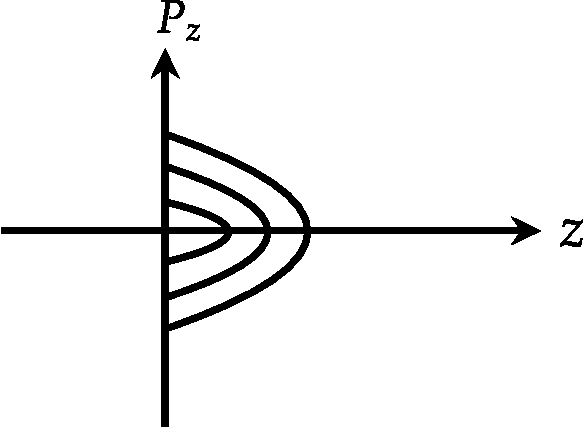
\includegraphics[height=3cm,width=5cm]{diagram-20210926(3)-crop}
	\end{figure}
	\task[\textbf{B.}]\begin{figure}[H]
		\centering
		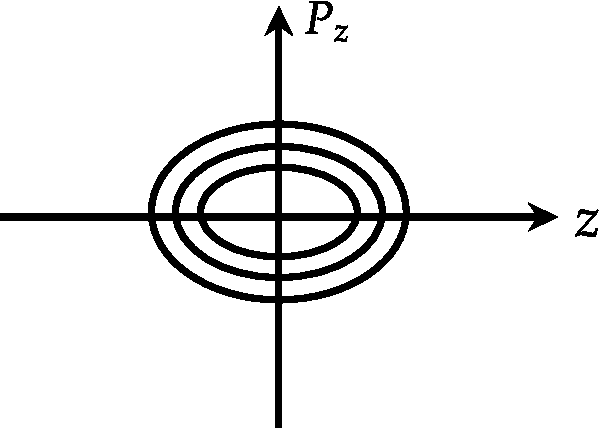
\includegraphics[height=3cm,width=5cm]{diagram-20210926(4)-crop}
	\end{figure}
	\task[\textbf{C.}]\begin{figure}[H]
		\centering
		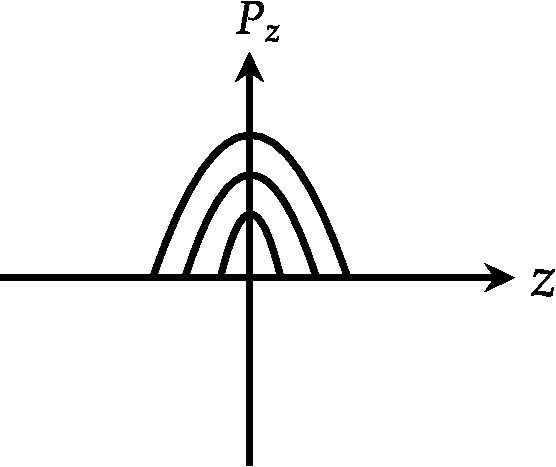
\includegraphics[height=3cm,width=5cm]{diagram-20210926(5)-crop}
	\end{figure}
	\task[\textbf{D.}]\begin{figure}[H]
		\centering
		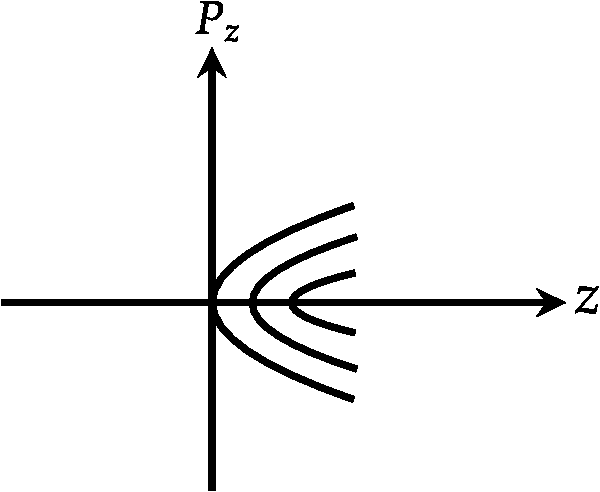
\includegraphics[height=3cm,width=5cm]{diagram-20210926(6)-crop}
	\end{figure}
\end{tasks}
\begin{answer}
	$$H=\frac{P_{z}^{2}}{2 m}+m g z \text { and } E=\frac{P_{z}^{2}}{2 m}+m g z$$
	The correct option is \textbf{(a)}
\end{answer}
\begin{minipage}{\textwidth}
	\item The bob of a simple pendulum, which undergoes small oscillations, is immersed in water. Which of the following figures best represents the phase space diagram for the pendulum?
	\exyear{NET JUNE 2012}
\end{minipage}
\begin{tasks}(2)
	\task[\textbf{A.}]\begin{figure}[H]
		\centering
		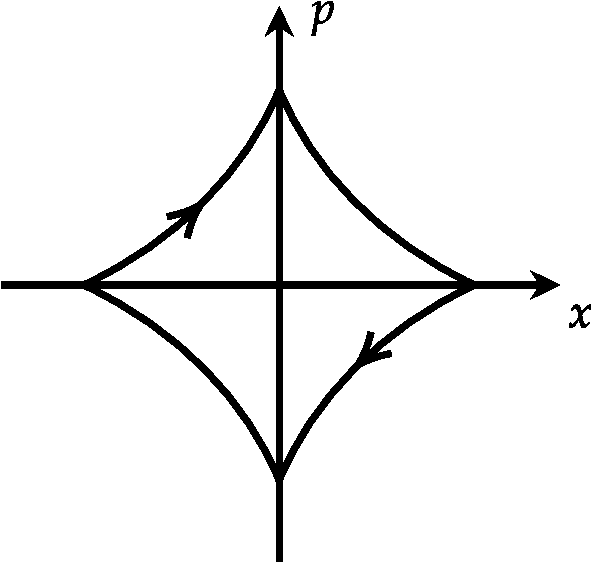
\includegraphics[height=3cm,width=5cm]{diagram-20210926(7)-crop}
	\end{figure}
	\task[\textbf{B.}]\begin{figure}[H]
		\centering
		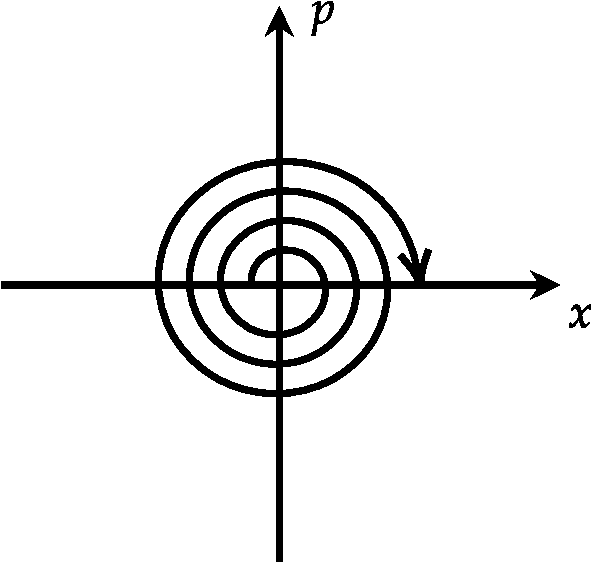
\includegraphics[height=3cm,width=5cm]{diagram-20210926(8)-crop}
	\end{figure}
	\task[\textbf{C.}]\begin{figure}[H]
		\centering
		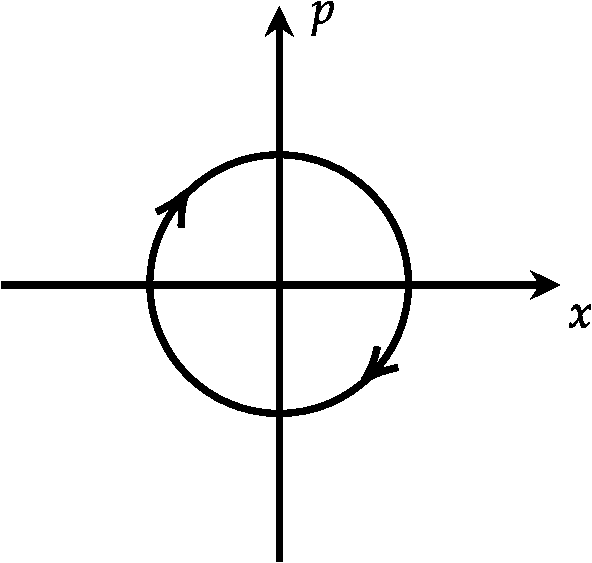
\includegraphics[height=3cm,width=5cm]{diagram-20210926(9)-crop}
	\end{figure}
	\task[\textbf{D.}]\begin{figure}[H]
		\centering
		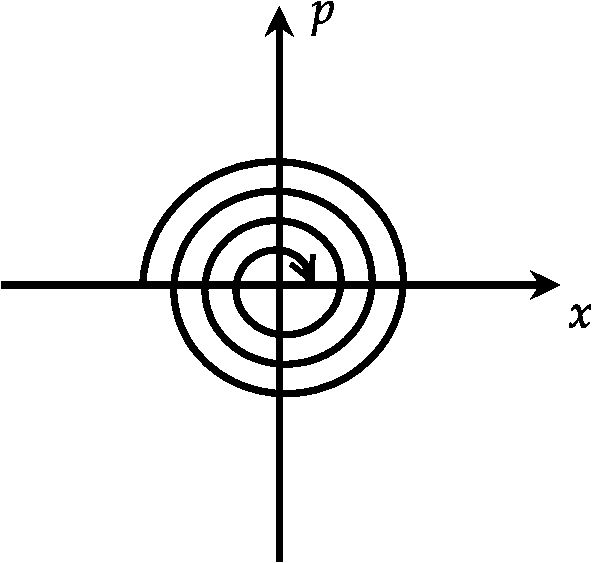
\includegraphics[height=3cm,width=5cm]{diagram-20210926(10)-crop}
	\end{figure}
\end{tasks}
\begin{answer}
 When simple pendulum oscillates in water it is damped oscillation so amplitude continuously decrease and finally it stops.\\
 The correct option \textbf{(d)}
\end{answer}
\begin{minipage}{\textwidth}
	\item Which of the following set of phase-space trajectories is not possible for a particle obeying Hamilton's equations of motion?
	\exyear{NET DEC 2012}
\end{minipage}
\begin{tasks}(2)
	\task[\textbf{A.}]\begin{figure}[H]
		\centering
		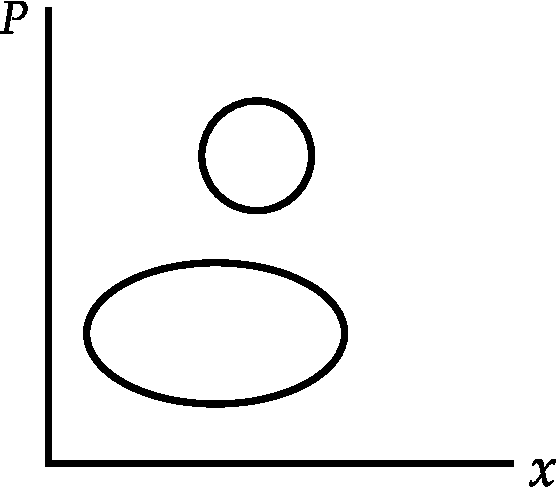
\includegraphics[height=3cm,width=5cm]{diagram-20210926(13)-crop}
	\end{figure}
	\task[\textbf{B.}]\begin{figure}[H]
		\centering
		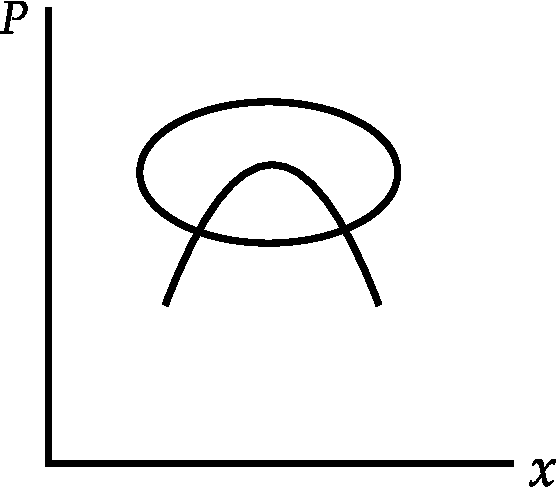
\includegraphics[height=3cm,width=5cm]{diagram-20210926(14)-crop}
	\end{figure}
	\task[\textbf{C.}]\begin{figure}[H]
		\centering
		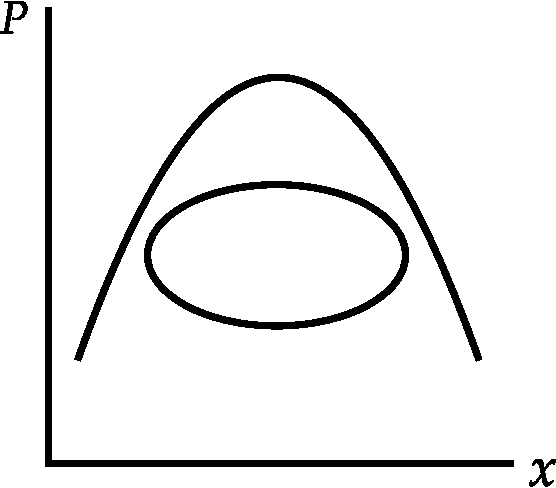
\includegraphics[height=3cm,width=5cm]{diagram-20210926(15)-crop}
	\end{figure}
	\task[\textbf{D.}]\begin{figure}[H]
		\centering
		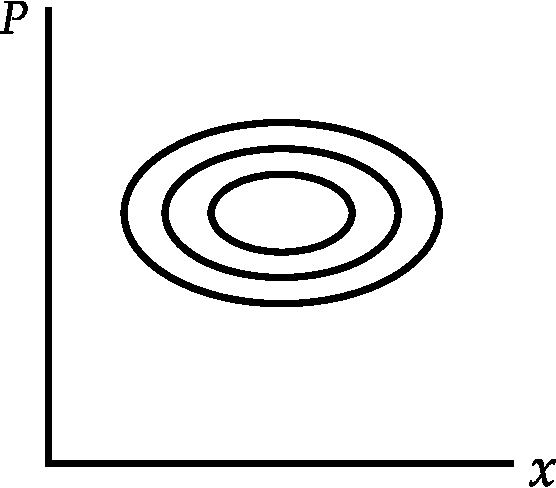
\includegraphics[height=3cm,width=5cm]{diagram-20210926(16)-crop}
	\end{figure}
\end{tasks}
\begin{answer}
 Phase curve does not cut each other \\
The correct option is \textbf{(b)}
\end{answer}
\begin{minipage}{\textwidth}
	\item The Hamiltonian of a classical particle moving in one dimension is $H=\frac{p^{2}}{2 m}+\alpha q^{4}$ where $\alpha$ is a positive constant and $p$ and $q$ are its momentum and position respectively. Given that its total energy $E \leq E_{0}$ the available volume of phase space depends on $E_{0}$ as
	\exyear{NET DEC 2014}
\end{minipage}
\begin{tasks}(2)
	\task[\textbf{A.}] $E_{0}^{3 / 4}$
	\task[\textbf{B.}]$E_{0}$
	\task[\textbf{C.}]$\sqrt{E_{0}}$
	\task[\textbf{D.}]is independent of $E_{0}$
\end{tasks}
\begin{answer}$\left. \right. $\\
\begin{minipage}{0.5\textwidth}
$H=\frac{p^{2}}{2 m}+\alpha q^{4}$
Phase area $=\oint p \cdot d q$
$$
\begin{aligned}
&A=\oint p \cdot d q=\pi \sqrt{2 m E} \times\left(\frac{E}{\alpha}\right)^{\frac{1}{4}} \\
&A \propto E_{0}^{1 / 2} \cdot E_{0}^{1 / 4} \Rightarrow A \propto E_{0}^{3 / 4}
\end{aligned}
$$	
\end{minipage}
\begin{minipage}{0.5\textwidth}
	\begin{figure}[H]
		\centering
		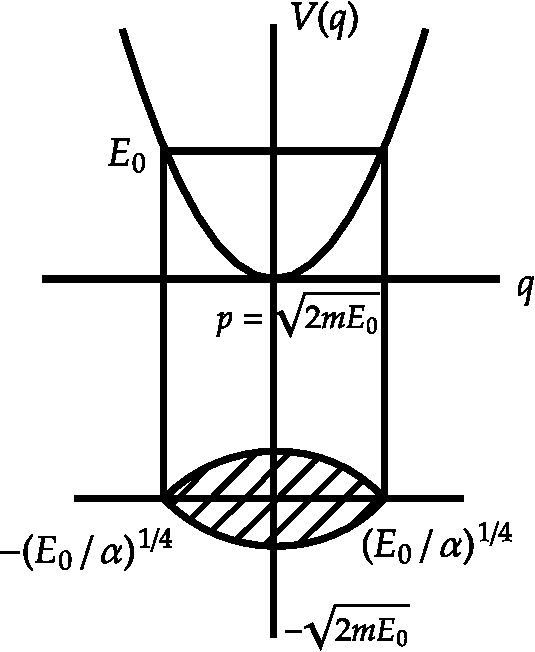
\includegraphics[height=5cm,width=5cm]{diagram-20210926(21)-crop}
	\end{figure}
\end{minipage}
The correct option is \textbf{(a)}	
\end{answer}
\begin{minipage}{\textwidth}
	\item Which of the following figures is a schematic representation of the phase space trajectories (i.e., contours of constant energy) of a particle moving in a one-dimensional potential $V(x)=\frac{-1}{2} x^{2}+\frac{1}{4} x^{4}$
	\exyear{NET JUNE 2015}
\end{minipage}
\begin{tasks}(2)
	\task[\textbf{A.}]\begin{figure}[H]
		\centering
		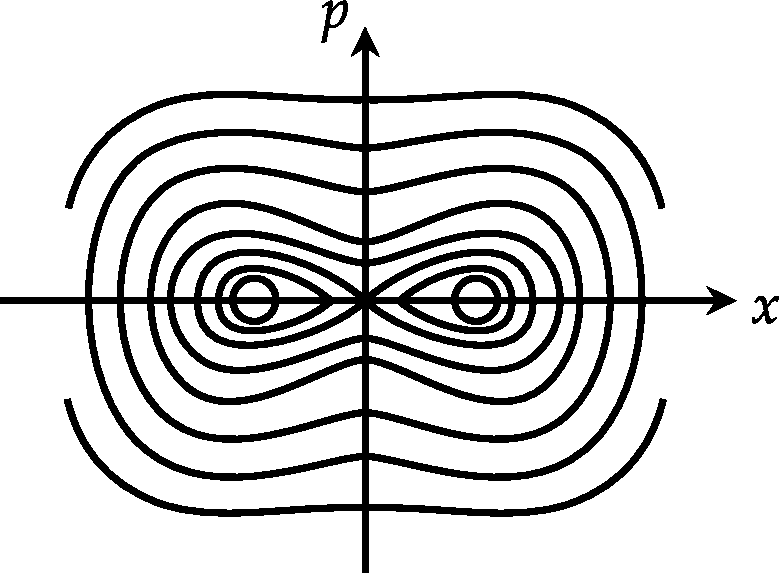
\includegraphics[height=3cm,width=5cm]{diagram-20210926(24)-crop}
	\end{figure}
	\task[\textbf{B.}]\begin{figure}[H]
		\centering
		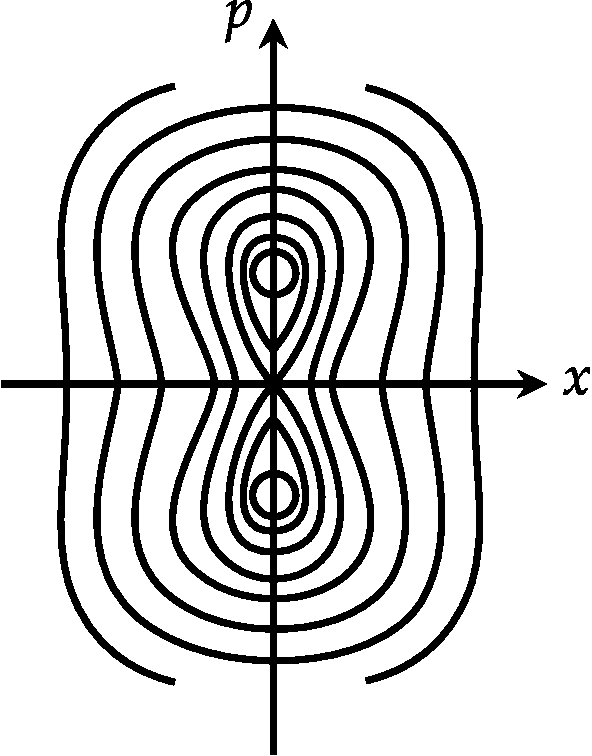
\includegraphics[height=3cm,width=5cm]{diagram-20210926(25)-crop}
	\end{figure}
	\task[\textbf{C.}]\begin{figure}[H]
		\centering
		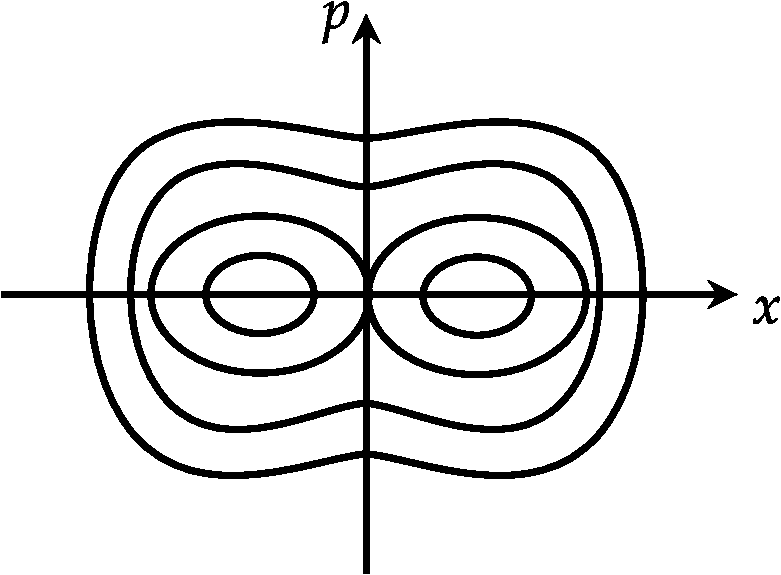
\includegraphics[height=3cm,width=5cm]{diagram-20210926(26)-crop}
	\end{figure}
	\task[\textbf{D.}]\begin{figure}[H]
		\centering
		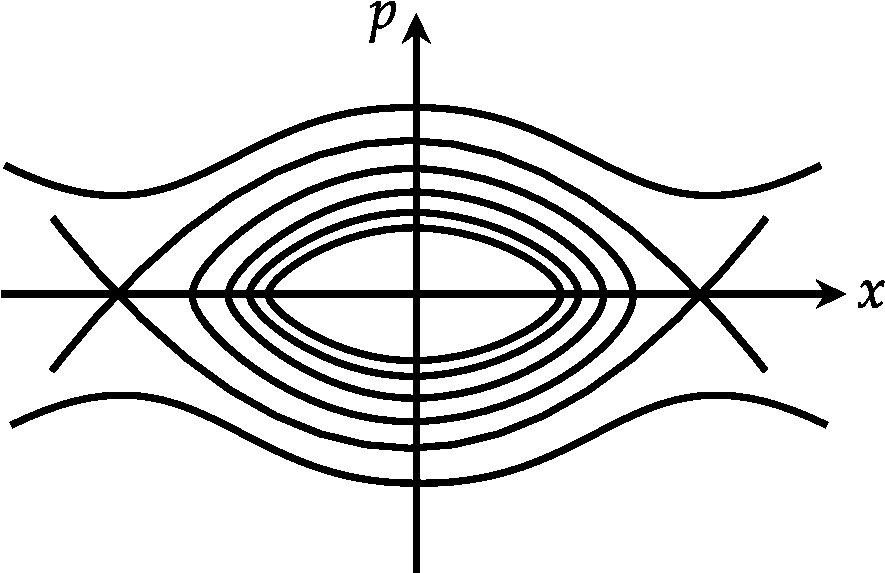
\includegraphics[height=3cm,width=5cm]{diagram-20210926(27)-crop}
	\end{figure}
\end{tasks}
\begin{answer}$\left. \right. $\\
	\begin{minipage}{0.5\textwidth}
	$V(x)=\frac{-x^{2}}{2}+\frac{x^{4}}{4}$
	$$
	\frac{\partial V}{\partial x}=0 \Rightarrow x=0, x=\pm 1
	$$
	$$
	\begin{aligned}
	&\frac{\partial^{2} V}{\partial x^{2}}=-v e \text { for } x=0 \text { (unstable point) } \\
	&=+\text { ve for } x=\pm 1 \text { (stable point) }
	\end{aligned}
	$$
	\end{minipage}
	\begin{minipage}{0.5\textwidth}
	\begin{figure}[H]
		\centering
		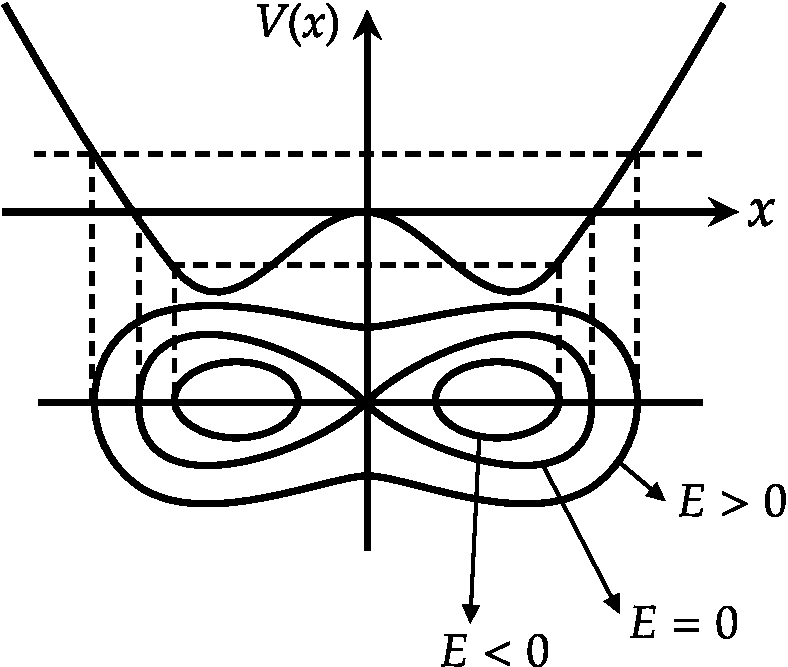
\includegraphics[height=5cm,width=5cm]{diagram-20210926(28)-crop(2)}
		\caption{}
		\label{}
	\end{figure}
	\end{minipage}
The correct option is \textbf{(a)}
\end{answer}
\begin{minipage}{\textwidth}
	\item A particle moves in one dimension in a potential $V(x)=-k^{2} x^{4}+\omega^{2} x^{2}$ where $k$ and $\omega$ are constants. Which of the following curves best describes the trajectories of this system in phase space?
	\exyear{NET DEC 2017}
\end{minipage}
\begin{tasks}(2)
	\task[\textbf{A.}]\begin{figure}[H]
		\centering
		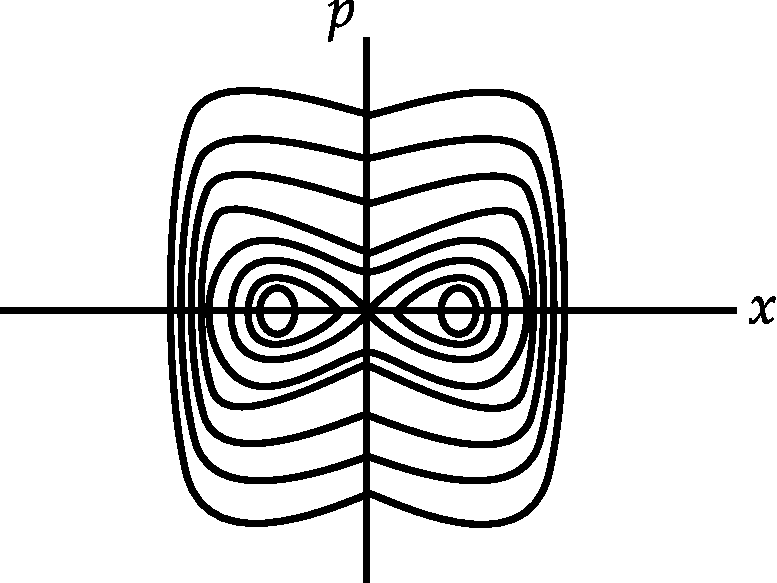
\includegraphics[height=3cm,width=5cm]{diagram-20210926(42)-crop}
	\end{figure}
	\task[\textbf{B.}]\begin{figure}[H]
		\centering
		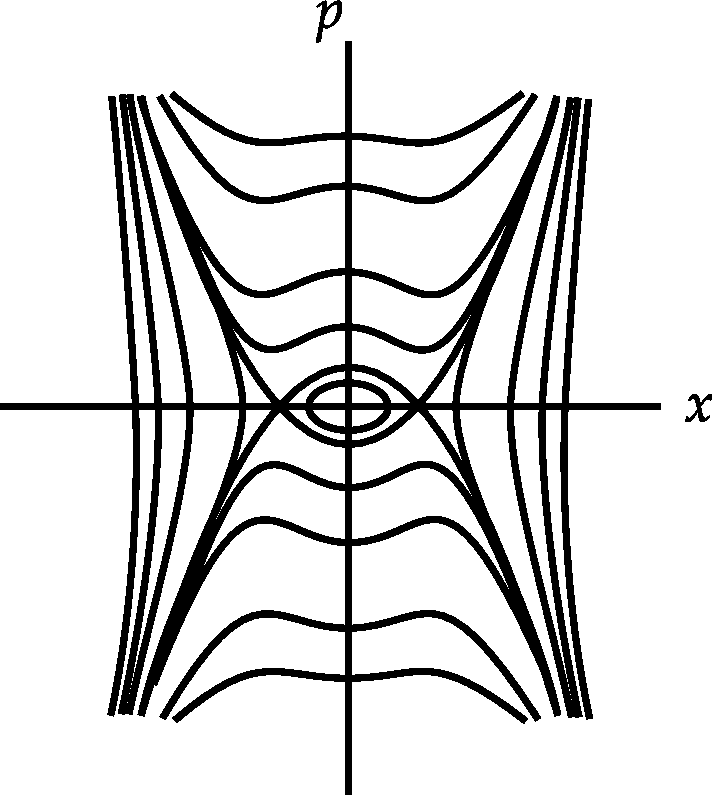
\includegraphics[height=3cm,width=5cm]{diagram-20210926(43)-crop}
	\end{figure}
	\task[\textbf{C.}]\begin{figure}[H]
		\centering
		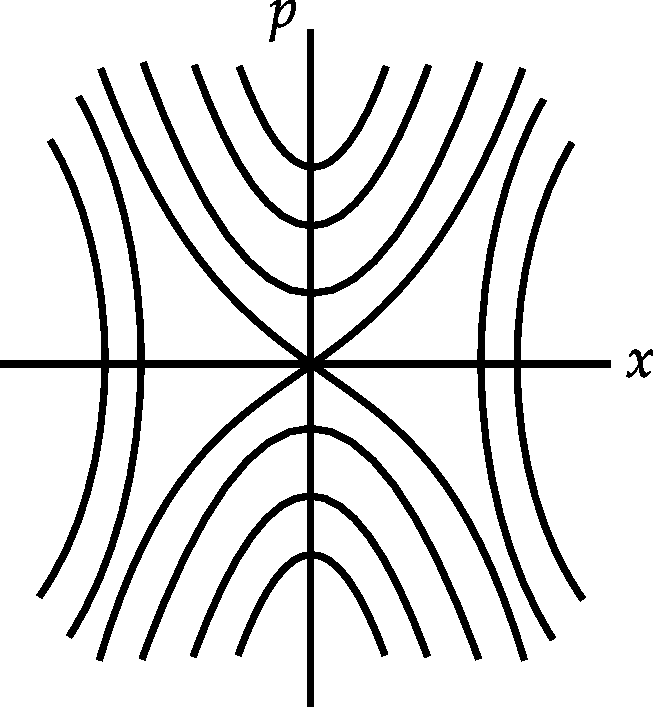
\includegraphics[height=3cm,width=5cm]{diagram-20210926(44)-crop}
	\end{figure}
	\task[\textbf{D.}]\begin{figure}[H]
		\centering
		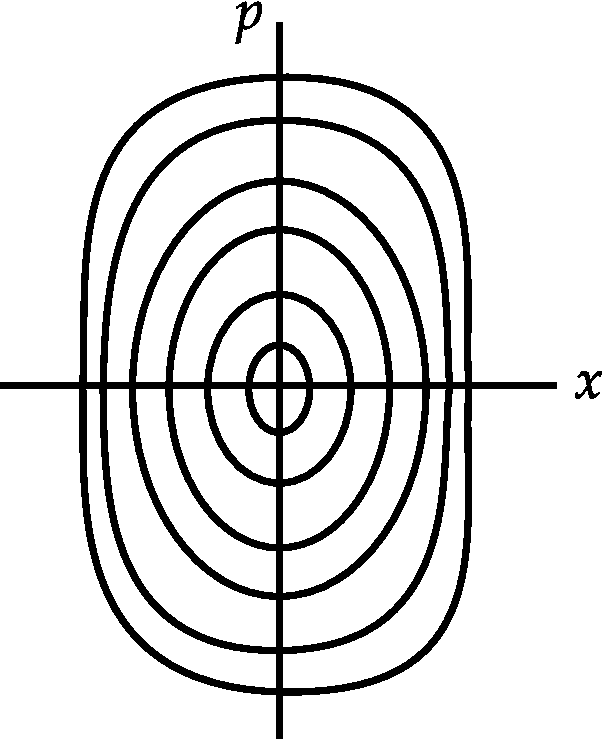
\includegraphics[height=3cm,width=5cm]{diagram-20210926(45)-crop}
	\end{figure}
\end{tasks}
\begin{answer}$\left. \right. $\\
	\begin{minipage}{0.5\textwidth}
	$V(x)=-k^{2} x^{4}+\omega^{2} x^{2}$\\
	For equation point\\
	$
	\frac{\partial V}{\partial x}=0 \Rightarrow-4 k^{2} x^{3}+2 \omega^{2} x=0, x=0 \text { or } x^{2}=\frac{\omega^{2}}{2 k^{2}}
	$\\
	Now, $\frac{d^{2} V}{d x^{2}}=-12 k^{2} x^{2}+2 \omega^{2}$ At, $x=0$\\
	$\frac{d^{2} V}{d x^{2}}=2 \omega^{2}, x=0$ is minimum.\\
	And, $\frac{d^{2} V}{d x^{2}}=-12 k^{2} \frac{\omega^{2}}{2 k^{2}}+2 \omega^{2}=-4 \omega^{2}$, at $x^{2}=\frac{\omega^{2}}{2 k^{2}}$\\
	Hence, $x=\pm \sqrt{\frac{\omega^{2}}{2 k^{2}}}$ is maxima.
	\end{minipage}
	 \begin{minipage}{0.5\textwidth}
	 \begin{figure}[H]
	 	\centering
	 	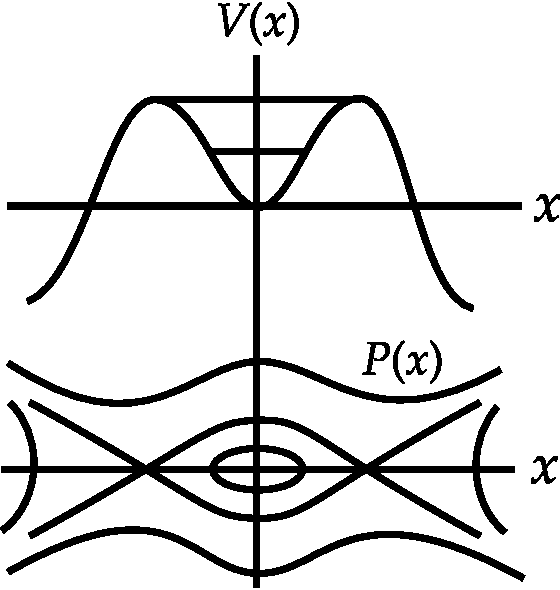
\includegraphics[height=4cm,width=5cm]{diagram-20210926(46)-crop}
	 \end{figure}
	 \end{minipage}
 The correct option is \textbf{(c)}
\end{answer}
\end{enumerate}
\newpage
\begin{abox}
	Practice set 2 solutions
	\end{abox}
\begin{enumerate}
\begin{minipage}{\textwidth}
	\item The Hamiltonian of particle of mass $m$ is given by $H=\frac{p^{2}}{2 m}-\frac{\alpha q^{2}}{2}$. Which one of the following figure describes the motion of the particle in phase space?
	\exyear{GATE 2014}
\end{minipage}
\begin{tasks}(2)
	\task[\textbf{A.}]\begin{figure}[H]
		\centering
		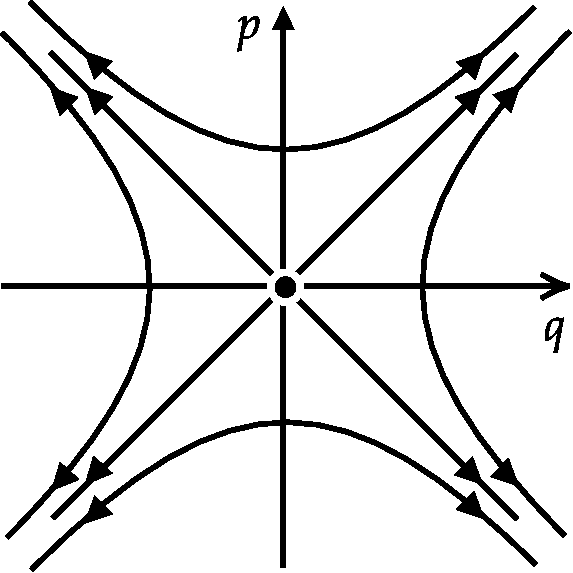
\includegraphics[height=4cm,width=5cm]{diagram-20210915(5)-crop}
	\end{figure}
	\task[\textbf{B.}]\begin{figure}[H]
		\centering
		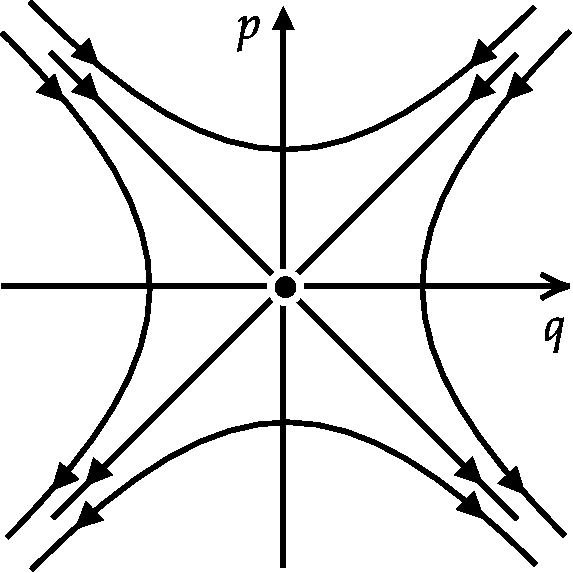
\includegraphics[height=4cm,width=5cm]{diagram-20210915(6)-crop}
	\end{figure}
	\task[\textbf{C.}]\begin{figure}[H]
		\centering
		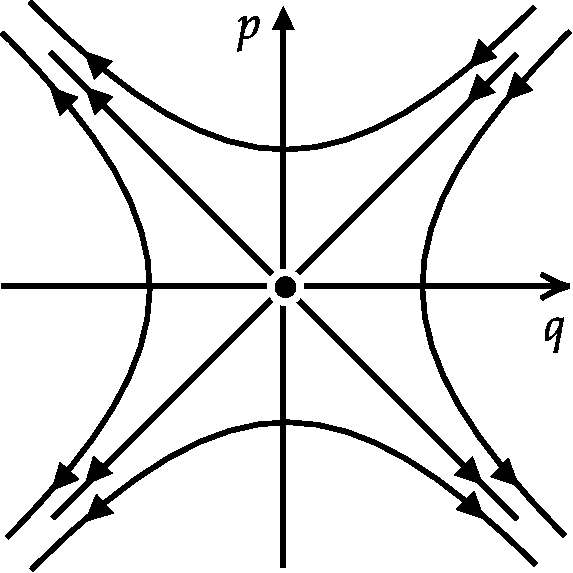
\includegraphics[height=4cm,width=5cm]{diagram-20210915(7)-crop}
	\end{figure}
	\task[\textbf{D.}]\begin{figure}[H]
		\centering
		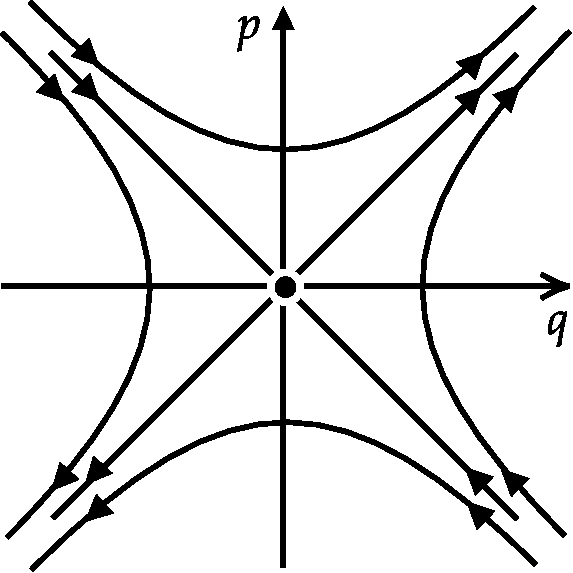
\includegraphics[height=4cm,width=5cm]{diagram-20210915(8)-crop}
	\end{figure}
\end{tasks}
\begin{answer}
	The corrrect option is \textbf{(d)}
\end{answer}
\begin{minipage}{\textwidth}
	\item A particle moves in one dimension under a potential $V(x)=\alpha|x|$ with some non-zero total energy. Which one of the following best describes the particle trajectory in the phase space?
	\exyear{GATE 2018}
\end{minipage}
\begin{tasks}(2)
	\task[\textbf{A.}]\begin{figure}[H]
		\centering
		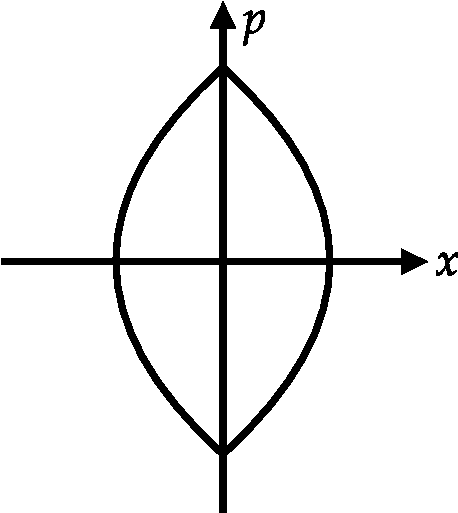
\includegraphics[height=3cm,width=5cm]{diagram-20210915(11)-crop}
	
	\end{figure}
	\task[\textbf{B.}]\begin{figure}[H]
		\centering
		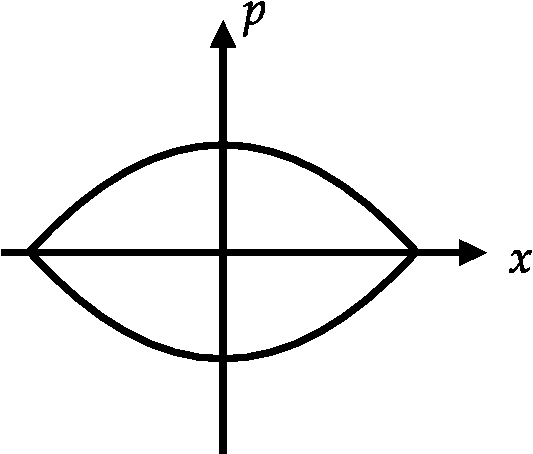
\includegraphics[height=3cm,width=5cm]{diagram-20210915(12)-crop}
	\end{figure}
	\task[\textbf{C.}]\begin{figure}[H]
		\centering
		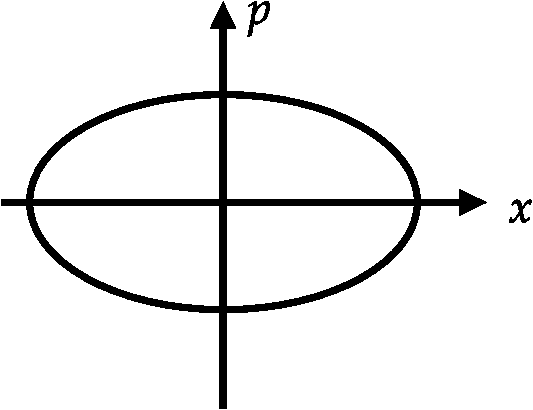
\includegraphics[height=3cm,width=5cm]{diagram-20210915(13)-crop}
	\end{figure}
	\task[\textbf{D.}]\begin{figure}[H]
		\centering
		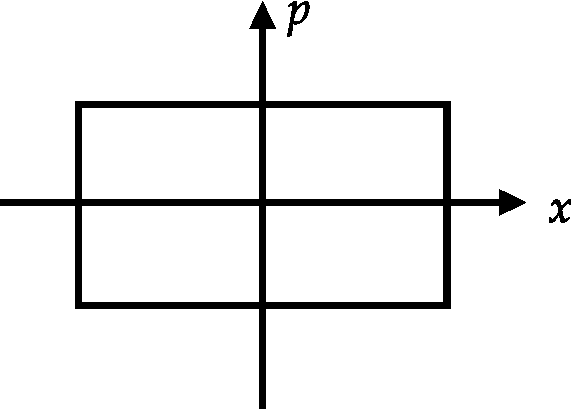
\includegraphics[height=3cm,width=5cm]{diagram-20210915(14)-crop}
	\end{figure}
\end{tasks}
\begin{answer}$\left. \right. $\\
\begin{minipage}{0.5\textwidth}
 $E=\frac{p^{2}}{2 m}+\alpha|x|$
	For $x>0, E=\frac{p^{2}}{2 m}+\alpha x$ $\Rightarrow p^{2}=2 m(E-\alpha x)$
	For $x<0, E=\frac{p^{2}}{2 m}-\alpha x$ $\Rightarrow p^{2}=2 m(E+\alpha x)$
\end{minipage}
\begin{minipage}{0.5\textwidth}
\begin{figure}[H]
	\centering
	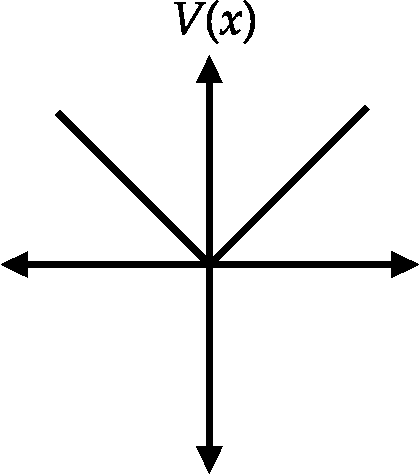
\includegraphics[height=3cm,width=4cm]{diagram-20210915(15)-crop}
\end{figure}
\begin{figure}[H]
	\centering
	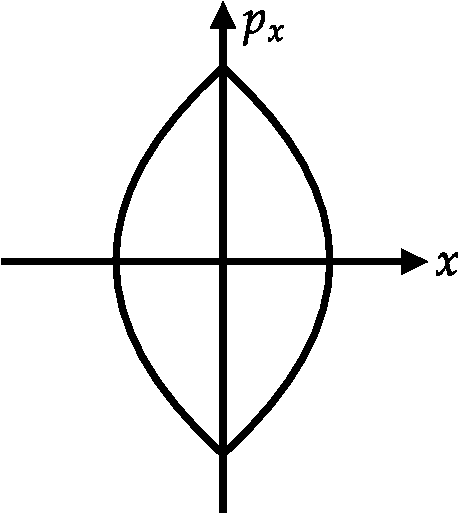
\includegraphics[height=3cm,width=5cm]{diagram-20210915(16)-crop}
\end{figure}
\end{minipage}
The correct option is \textbf{(a)}	
\end{answer}
\begin{minipage}{\textwidth}
	\item A ball bouncing of a rigid floor is described by the potential energy function
	$$
	V(x)=\left\{\begin{array}{lll}
	m g x & \text { for } & x>0 \\
	\infty & \text { for } & x \leq 0
	\end{array}\right.
	$$
	Which of the following schematic diagrams best represents the phase space plot of the ball?
	\exyear{GATE 2019}
\end{minipage}
\begin{tasks}(2)
	\task[\textbf{A.}]\begin{figure}[H]
		\centering
		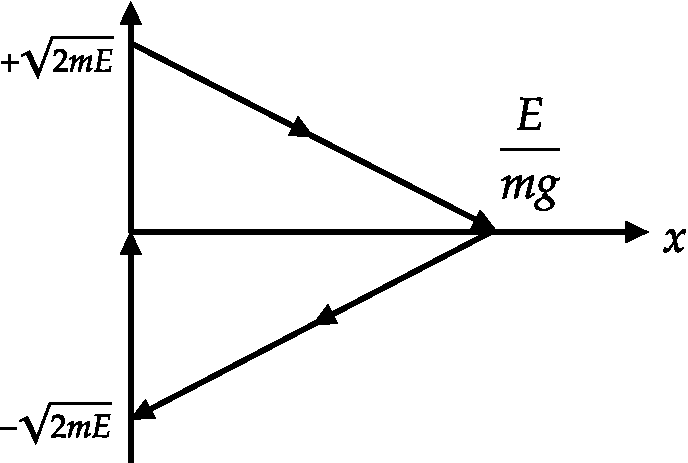
\includegraphics[height=3cm,width=5cm]{diagram-20210915(18)-crop}
	\end{figure}
	\task[\textbf{B.}]\begin{figure}[H]
		\centering
		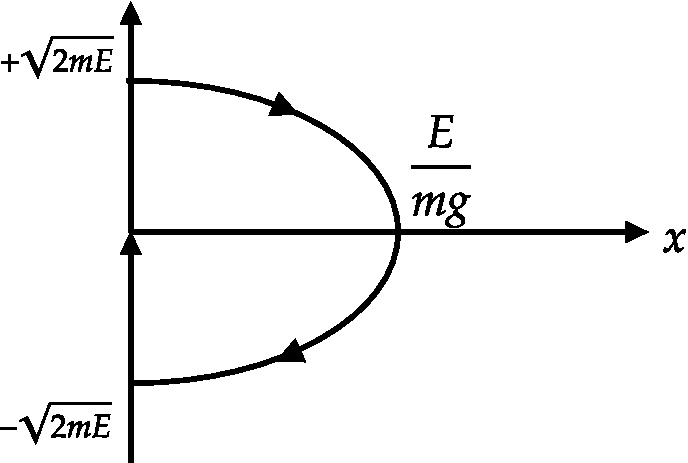
\includegraphics[height=3cm,width=5cm]{diagram-20210915(19)-crop}
	\end{figure}
	\task[\textbf{C.}]\begin{figure}[H]
		\centering
		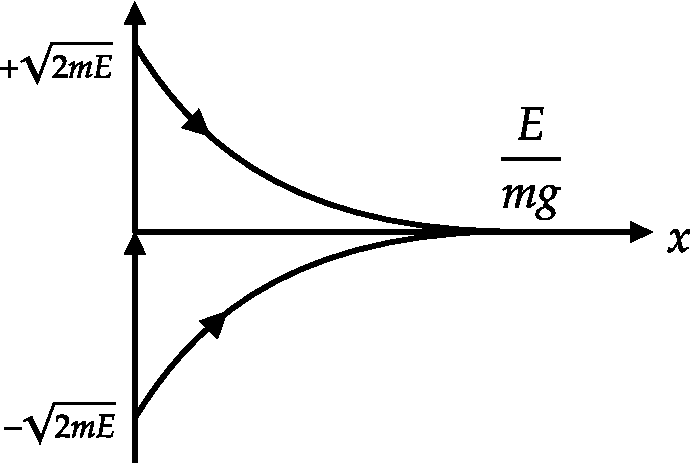
\includegraphics[height=3cm,width=5cm]{diagram-20210915(20)-crop}
	\end{figure}
	\task[\textbf{D.}]\begin{figure}[H]
		\centering
		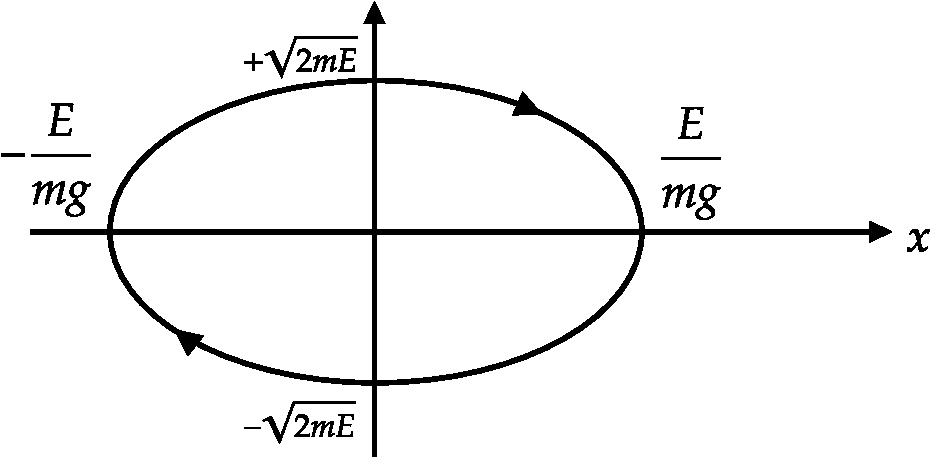
\includegraphics[height=3cm,width=5cm]{diagram-20210915(21)-crop}
	\end{figure}
\end{tasks}
\begin{answer}
	$E=\frac{p^{2}}{2 m}+m g x \Rightarrow p^{2}=2 m(E-m g x) \text { which is equation of parabola }$\\
	The correct option is \textbf{(b)}
\end{answer}
\end{enumerate}